\documentclass{reportkit}
% Local to this report only (not a core-file change): force tables/figures
% to stay exactly where placed in source rather than drifting to the top of
% a page ahead of the section text that introduces them.
\usepackage{float}

\setreportkitleftheader{CAREER DEVELOPMENT / PRACTITIONER GUIDE}
\setreportkitfooter{Professional Career Exploration Framework}
\setreportkitversion{v1.0}

\title{The Professional Career Exploration Framework}
\author{Career Development Practice}
\date{4 September 2026}

\begin{document}
\maketitle

\begin{execsummary}
Career preparation fails most often not from a lack of effort but from treating it as
a linear sequence -- pick a career, take courses, apply for jobs -- rather than as a
system with feedback. This guide reframes career exploration as a cycle: research the
market, model the competencies it actually rewards, assess the resulting gap,
close it through skill acquisition and evidence-building, gain professional exposure,
enter recruitment, and use the outcomes to update the underlying career hypothesis.
The central claim is multiplicative rather than additive: strong technical skills
cannot compensate for weak evidence, and a polished portfolio cannot compensate for
undeveloped interview skill. Any single weak link becomes the binding constraint on
readiness, so the framework is built around eight living artifacts a student
maintains and revises throughout, not a one-time plan.
\end{execsummary}

\section{A system, not a sequence}
Treat career preparation as \emph{research $\to$ capability $\to$ evidence $\to$
recruitment $\to$ feedback}, applicable across data engineering, consulting, finance,
product management, cybersecurity, marketing, UX, and operations alike -- only the
content inside each stage changes by profession.

A useful way to make the multiplicative structure explicit:

\begin{equation}
  \mathrm{CR} = D \times C \times E \times A \times R,
  \label{eq:readiness}
\end{equation}

where $D$ is direction (a tested career hypothesis), $C$ is capability, $E$ is
evidence, $A$ is access to the hiring ecosystem, and $R$ is recruitment skill
(applications and interviewing). Equation~\ref{eq:readiness} is deliberately
multiplicative: someone can have excellent technical skills but weak evidence,
excellent credentials but no understanding of recruitment, or a superb portfolio but
consistently fail interviews. Any one near-zero factor caps the product.

\begin{principle}{Career engineering, not career counselling}
Teach the process as formulating hypotheses, collecting market evidence, running
experiments, building capabilities, demonstrating them, testing them against the
labour market, diagnosing failures, and iterating -- not as one-time advice-giving.
\end{principle}

\section{Career discovery and market research}

\subsection{What does the profession actually involve?}
Before acquiring skills, a student needs an accurate mental model of the occupation.
Table~\ref{tab:discovery} lists the dimensions worth triangulating across job
descriptions, professional associations, practitioners, career pages, LinkedIn
profiles, salary surveys, and informational interviews.

\begin{table}[H]
\caption{Career discovery dimensions and outputs}
\label{tab:discovery}
\centering
\begin{tabular}{ll}
\toprule
Dimension & Student output \\
\midrule
Role definition & 1-page role brief \\
Role variants & Career map \\
Employers & 20--30 target employers \\
Industries & Industry map \\
Seniority progression & Progression ladder \\
Compensation & Compensation benchmark \\
Lifestyle (hours, travel, WFH) & Lifestyle assessment \\
Geography & Geographic assessment \\
Future outlook & Opportunity/risk assessment \\
\bottomrule
\end{tabular}
\source{Practitioner-derived discovery framework.}
\end{table}

\begin{deliverablenote}{Career Hypothesis}
``I think I want to become X because of A/B/C. The work appears to involve D/E/F.
Before committing, I need to test assumptions G/H/I.'' Stating the hypothesis this
way, with its own open assumptions attached, is what prevents premature commitment.
\end{deliverablenote}

\subsection{Recruitment reverse engineering}
Research recruitment itself as a data-collection exercise rather than relying on
generic career advice. Collect 30--50 representative job advertisements and extract
technical requirements (tools, technologies, methodologies, certifications, domain
knowledge), behavioural requirements (communication, leadership, stakeholder
management, problem solving, teamwork, commercial awareness), and experience signals
(internships, projects, research, prior industries, leadership activity). Calculating
approximate frequency across the sample turns generic advice into a market-derived
competency model, illustrated in Figure~\ref{fig:frequency}.

\begin{figure}[H]
  \centering
  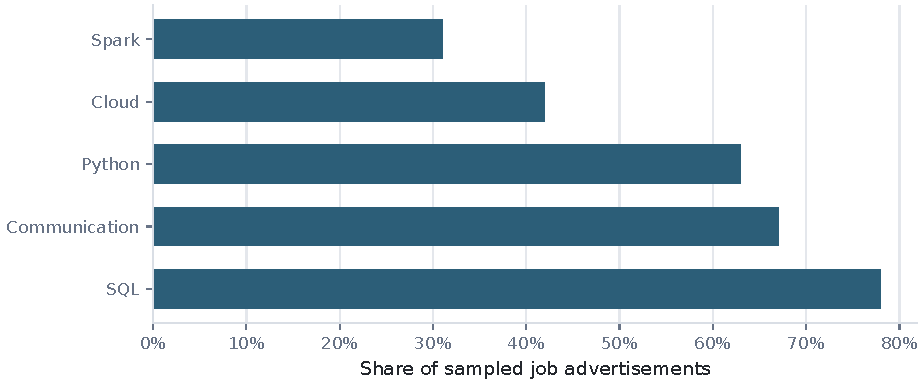
\includegraphics[width=\linewidth]{figures/competency_frequency.pdf}
  \caption{Illustrative competency frequency across a sample of job advertisements.}
  \label{fig:frequency}
  \source{Illustrative values matching the worked example in the source framework; a
  real analysis should use the student's own sampled advertisements.}
\end{figure}

Separately, map the recruitment funnel itself -- application, screening, assessment,
interview, technical or case exercise, final interview, offer -- and for each stage
determine what is being assessed, how it is assessed, what strong performance looks
like, and what causes candidates to fail.

\begin{deliverablenote}{Recruitment Map and Competency Matrix}
A market-derived list of required competencies with approximate frequencies, plus a
stage-by-stage map of what each part of the recruitment funnel actually tests.
\end{deliverablenote}

\section{Self-assessment}
Compare the student against the competency model. A useful scoring pattern is
competency, market importance, current level, evidence, and the resulting gap
(Table~\ref{tab:gap}).

\begin{table}[H]
\caption{Illustrative capability gap analysis}
\label{tab:gap}
\centering
\begin{tabular}{lS[table-format=1.0]S[table-format=1.0]lS[table-format=1.0]}
\toprule
Competency & {Market importance} & {Current level} & Evidence & {Gap} \\
\midrule
SQL              & 5 & 3 & University project & 2 \\
Python            & 5 & 4 & Internship         & 1 \\
Cloud             & 3 & 1 & None               & 2 \\
Communication     & 4 & 3 & Presentations      & 1 \\
Domain knowledge  & 4 & 2 & Coursework         & 2 \\
\bottomrule
\end{tabular}
\source{Illustrative self-assessment; scale is 1 (low) to 5 (high).}
\end{table}

\begin{limitationnote}{Self-rated competence is weak evidence on its own}
``I completed a Python course'' and ``I independently built and deployed a Python
application used by 30 people'' are fundamentally different claims. The evidence
column in Table~\ref{tab:gap} should distinguish exposure, knowledge, application,
independent execution, and professional competence rather than a single self-rating.
\end{limitationnote}

\begin{diagram}[
  type=network,
  caption={Competence deepens through five stages; only the later stages constitute strong recruitment evidence.},
  label={fig:competence},
  source={Illustrative conceptual progression.},
  description={Five stages in sequence: exposure, knowledge, application, independent execution, professional competence.}
]
  \RKNode[text width=19mm]{exposure}{0.3}{0}{Exposure}
  \RKNode[text width=19mm]{knowledge}{3.6}{0}{Knowledge}
  \RKNode[text width=19mm]{application}{6.9}{0}{Application}
  \RKNode[text width=19mm]{independent}{10.2}{0}{Independent\\execution}
  \RKNode[rk accent,text width=19mm]{professional}{13.5}{0}{Professional\\competence}
  \RKEdge{sequence}{exposure}{knowledge}
  \RKEdge{sequence}{knowledge}{application}
  \RKEdge{sequence}{application}{independent}
  \RKEdge{sequence}{independent}{professional}
\end{diagram}

\begin{deliverablenote}{Personal Capability Gap Analysis}
A scored comparison of the student against the market-derived competency model, with
evidence type recorded per competency, not just a numeric self-rating.
\end{deliverablenote}

\section{Skill acquisition}
Students should not simply accumulate courses. A useful progression is learn, practice,
apply, integrate, demonstrate (Figure~\ref{fig:acquisition}). Integration matters
specifically: a data engineering student combining Python, SQL, Docker, cloud, and
orchestration into one working system builds more capability than five unrelated
tutorials.

\begin{diagram}[
  type=network,
  caption={Skill acquisition progression.},
  label={fig:acquisition},
  source={Illustrative conceptual progression.},
  description={Five stages in sequence: learn, practice, apply, integrate, demonstrate.}
]
  \RKNode[text width=19mm]{learn}{0.3}{0}{Learn}
  \RKNode[text width=19mm]{practice}{3.6}{0}{Practice}
  \RKNode[text width=19mm]{apply}{6.9}{0}{Apply}
  \RKNode[text width=19mm]{integrate}{10.2}{0}{Integrate}
  \RKNode[rk accent,text width=19mm]{demonstrate}{13.5}{0}{Demonstrate}
  \RKEdge{sequence}{learn}{practice}
  \RKEdge{sequence}{practice}{apply}
  \RKEdge{sequence}{apply}{integrate}
  \RKEdge{sequence}{integrate}{demonstrate}
\end{diagram}

\begin{principle}{Courses build capability; evidence communicates capability}
A completed course is necessary but not sufficient. The demonstration stage --
producing something another person can evaluate -- is what recruitment actually
tests.
\end{principle}

\section{Project and portfolio development}
Projects should progressively resemble professional work (Figure~\ref{fig:projects}).
Guided tutorials teach mechanics but are weak portfolio evidence; professionally
realistic projects introduce the constraints practitioners actually encounter --
incomplete requirements, messy data, cost constraints, stakeholders, performance
requirements, documentation, deployment, and trade-offs.

\begin{diagram}[
  type=network,
  caption={Project realism should escalate rather than accumulate.},
  label={fig:projects},
  source={Illustrative conceptual progression.},
  description={Five levels in sequence: guided, modified, independent, professionally realistic, externally validated.}
]
  \RKNode[text width=19mm]{guided}{0.3}{0}{Guided}
  \RKNode[text width=19mm]{modified}{3.6}{0}{Modified}
  \RKNode[text width=19mm]{independent}{6.9}{0}{Independent}
  \RKNode[text width=19mm]{realistic}{10.2}{0}{Professionally\\realistic}
  \RKNode[rk accent,text width=19mm]{validated}{13.5}{0}{Externally\\validated}
  \RKEdge{sequence}{guided}{modified}
  \RKEdge{sequence}{modified}{independent}
  \RKEdge{sequence}{independent}{realistic}
  \RKEdge{sequence}{realistic}{validated}
\end{diagram}

\subsection{Communicating what a project accomplished}
A technically impressive project is still weak recruitment evidence if no one can
understand what it accomplished. Every major project should communicate its problem,
context, constraints, approach, decisions, implementation, results, and reflection --
this structure also produces the raw material for resumes and interviews directly.
Portfolio format itself is profession-specific: GitHub for software or data roles,
investment reports for finance, case studies for consulting, design case studies for
UX, campaigns and analytics for marketing, CAD or design portfolios for engineering.

\subsection{The career evidence stack}
Evidence accumulates in strength as it becomes rarer (Figure~\ref{fig:evidencestack}).
A credential is common and cheap to obtain; a measured, externally validated outcome
is rare and difficult to fabricate. This is why another certificate is not necessarily
the highest-value next step once the lower tiers are already covered.

\begin{diagram}[
  type=stack,
  caption={The career evidence stack.},
  label={fig:evidencestack},
  source={Illustrative progression; ordering reflects persuasiveness to a recruiter, not a measured population.},
  description={Seven tiers rising from credential through measured impact, each narrower and rarer than the one below it.}
]
  \RKStackSetup{12}{0.95}{7}
  \RKStackTier{0}{Credential --- ``I studied machine learning''}
  \RKStackTier{1}{Assessment --- scored well in the subject}
  \RKStackTier{2}{Project --- built a machine-learning system}
  \RKStackTier{3}{Demonstrated complexity --- deployed to AWS, designed monitoring}
  \RKStackTier{4}{External validation --- other people used it}
  \RKStackTier[rk accent]{5}{Professional experience --- operated similar systems in an internship}
  \RKStackTier{6}{Measured impact --- reduced processing time by 40\%}
\end{diagram}

\begin{deliverablenote}{Evidence Portfolio}
Projects, internships, and demonstrated competencies, each tagged with which tier of
Figure~\ref{fig:evidencestack} it actually reaches -- not just a list of things
completed.
\end{deliverablenote}

\section{Professional experience and network}
Projects experience diminishing returns on their own. Students should actively seek
increasingly authentic environments: classroom, student organisation, competition,
external project, internship, professional work. Channels include internships,
apprenticeships, research assistantships, hackathons, case competitions, consulting
projects, volunteering, open-source contributions, professional societies, and
university-industry collaborations. The objective is exposure to professional
constraints and standards, not merely filling a resume line.

Networking is information-gathering and relationship development, not transactional
referral requests. Identify peers (entering similar careers), near-peers (graduates
1--3 years ahead, often the most useful because they recently went through
recruitment), practitioners currently doing the job, and the hiring ecosystem
(recruiters, managers, associations, alumni). Informational interviews should
directly test the career hypothesis from Section~2: what does a normal week look
like, what surprised you after joining, what actually distinguishes strong juniors,
what does recruitment test, and what do students typically misunderstand about the
role. Update the career hypothesis based on what comes back.

\section{Application engineering and interview capability}
Applications are their own skill. Resumes should read as experience $\to$ action
$\to$ difficulty/scale $\to$ outcome rather than restated job descriptions.
Opportunities should be separated into reach, target, and safety tiers and tracked
across company, position, deadline, application status, referral, stage, outcome, and
feedback. Signalling should stay aligned across resume, portfolio, LinkedIn, and
interview narrative so the candidate tells one coherent professional story.

Interview preparation decomposes into distinct skills rather than one undifferentiated
skill (Table~\ref{tab:interview}).

\begin{table}[H]
\caption{Interview preparation by category}
\label{tab:interview}
\centering
\begin{tabular}{lp{7.6cm}}
\toprule
Category & What to practise \\
\midrule
Behavioural & Build an experience bank of 8--12 significant experiences recorded as
  situation, objective, actions, decisions, challenges, result, and learning -- not
  memorised scripts. \\
Technical & Identify the profession-specific format: coding, SQL, modelling, system
  design, accounting, financial analysis, statistics, or engineering problems. \\
Case / problem-solving & Structure, assumptions, analysis, synthesis,
  recommendation. \\
Communication & Explain the same concept at specialist, manager, client, and
  non-specialist levels. \\
Mock interviews & Progress from untimed practice to timed practice, peer mock,
  expert mock, and realistic simulation; record and review specific failure
  modes. \\
\bottomrule
\end{tabular}
\end{table}

\begin{deliverablenote}{Application Tracker and Experience Bank}
A tracked list of applications by stage and outcome, and a structured bank of 8--12
experiences ready to answer multiple behavioural questions.
\end{deliverablenote}

\section{Recruitment analytics}
Applications generate data. Tracking conversion from applications through screens,
first interviews, final interviews, and offers turns rejection into diagnostic
information rather than an undifferentiated setback (Figure~\ref{fig:funnel},
Table~\ref{tab:diagnosis}).

\begin{diagram}[
  type=funnel,
  caption={Recruitment conversion narrows at every stage.},
  label={fig:funnel},
  source={Illustrative shape; a real analysis should use the student's own tracked conversion counts.},
  description={Five tapering stages: applications, screens, first interviews, final interviews, and offers.}
]
  \RKFunnelSetup{10.5}{1.1}
  \RKFunnelStage{0}{1.00}{0.62}{Applications}
  \RKFunnelStage{1}{0.62}{0.40}{Screens}
  \RKFunnelStage{2}{0.40}{0.24}{First interviews}
  \RKFunnelStage{3}{0.24}{0.13}{Final interviews}
  \RKFunnelStage[rk accent]{4}{0.13}{0.07}{Offers}
\end{diagram}

\begin{table}[H]
\caption{Diagnosing recruitment outcomes}
\label{tab:diagnosis}
\centering
\begin{tabular}{lp{7cm}}
\toprule
Observed pattern & Likely issue \\
\midrule
Almost no interviews & Targeting, resume, or experience \\
Screens but no technical rounds & Communication or basic fit \\
Repeated technical-round failures & Technical competence \\
Technical pass but final-round rejection & Behavioural fit or communication \\
Offers consistently unattractive & Targeting or market positioning \\
\bottomrule
\end{tabular}
\source{Illustrative diagnostic heuristics; conclusions should be checked against the student's own conversion data.}
\end{table}

\section{Experimentation and decision framework}
Career exploration should include inexpensive experiments before expensive
commitments. For each career hypothesis: research it (read about the profession),
observe it (speak to practitioners), simulate it (perform representative tasks),
experience it (internship, project, or shadowing), and evaluate it against fit,
enjoyment of the learning curve, lifestyle, market demand, and compensation.

\begin{decisionpoint}{Scoring competing career hypotheses}
Weight dimensions such as interest, aptitude, job availability, compensation,
progression, lifestyle, geographic fit, skill transferability, and future
resilience, and score each candidate career against them. The numbers are not
objectively correct -- their purpose is to expose assumptions and trade-offs the
student might otherwise leave implicit, especially where a career is being chosen
primarily for prestige or a superficial description.
\end{decisionpoint}

\section{The continuous feedback loop}
The complete framework is cyclical (Figure~\ref{fig:loop}), not a project with an
end state. Recruitment outcomes feed back into the competency model from
Section~2, which changes what gets prioritised in Section~4 and Section~5.

\begin{diagram}[
  type=cycle,
  caption={The career exploration feedback loop.},
  label={fig:loop},
  source={Illustrative conceptual cycle.},
  description={Six stages arranged in a ring, each connected to the next, looping back to the first: explore careers, research market, assess self, build evidence, enter recruitment, update hypothesis.}
]
  \RKCycleSetup{4.3}
  \RKCycleNode{explore}{90}{Explore\\careers}
  \RKCycleNode{research}{30}{Research\\market}
  \RKCycleNode{assess}{-30}{Assess\\self}
  \RKCycleNode[rk accent]{build}{-90}{Build\\evidence}
  \RKCycleNode{recruit}{-150}{Enter\\recruitment}
  \RKCycleNode{update}{150}{Update\\hypothesis}

  \RKCycleEdge{explore}{research}
  \RKCycleEdge{research}{assess}
  \RKCycleEdge{assess}{build}
  \RKCycleEdge{build}{recruit}
  \RKCycleEdge{recruit}{update}
  \RKCycleEdge[repeat]{update}{explore}
\end{diagram}

\section{The eight living artifacts}
To keep the framework usable rather than read once, operationalise it around eight
artifacts a student maintains and revises continuously (Table~\ref{tab:artifacts}).

\begin{table}[H]
\caption{The eight living artifacts}
\label{tab:artifacts}
\centering
\begin{tabular}{lp{7.6cm}}
\toprule
Artifact & Purpose \\
\midrule
Career Map & Roles currently being explored and why. \\
Market Dataset & 30--50 job advertisements and extracted requirements. \\
Competency Matrix & Required capabilities versus current evidence. \\
Learning Backlog & Prioritised skills and learning resources. \\
Evidence Portfolio & Projects, internships, and demonstrated competencies. \\
Experience Bank & Structured examples for behavioural interviews. \\
Application Tracker & Applications, stages, and outcomes. \\
Career Review & Periodic assessment of whether the career hypothesis still holds. \\
\bottomrule
\end{tabular}
\source{Practitioner-derived dashboard structure.}
\end{table}

\begin{researchproblem}{Which factor is binding?}
Given Equation~\ref{eq:readiness}, the recurring diagnostic question for any student
who is not converting is which factor -- direction, capability, evidence, access, or
recruitment skill -- is currently closest to zero, since that is the one worth
addressing next.
\end{researchproblem}

\end{document}
